%%Énoncé
On considère l’algorithme MYSHORTESTPATH pour trouver le plus court chemin
entre un sommet start et un sommet destination dans un graphe pondéré
connecté. Tous les poids sont supposés positifs et le graphe est supposé simple. \\


\begin{figure}[hp]
	\centering
		\vspace{-0.4cm}
		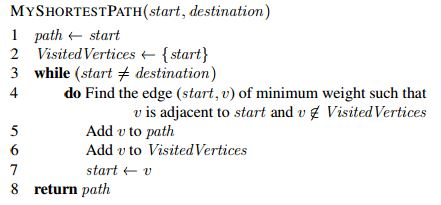
\includegraphics[scale=0.8]{MyShortestPath.JPG}
	\label{fig:MyShortestPath}
\end{figure}

L’algorithme MYSHORTESTPATH fonctionne-t-il toujours, jamais ou parfois seulement ? Argumentez 
%%Auteur
(Mathieu) \\
%%Réponse

L'algorithme présenté ci-dessus ne fonctionne pas toujours, mais il y a des cas où le résultat est correct. Par exemple dans le graphe ci-dessous, le chemin de poids minimum trouvé par l'algorithme entre A et E passe par les noeuds A-C-E pour un poids total de 12, alors que le chemin optimal est de 11 par les noeud A-D-E. D'autre part, si l'on cherche le chemin le plus court entre les noeuds D et B avec cet algorithme, on obtient le chemin D-E-B, qui est le chemin de poids le plus faible (poids total = 7).

\begin{figure}[hp]
	\centering
		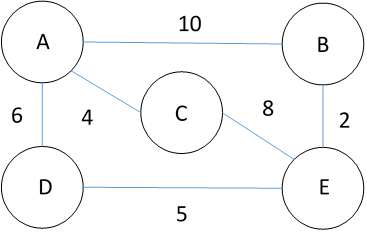
\includegraphics[scale=0.8]{Graph.png}
	\label{fig:Graph}
\end{figure}

Cet algorithme ne fonctionne pas car il est beaucoup trop simple, en effet il ne tient compte que d'un déplacement à la fois et ne tient pas compte des futurs chemins possibles/écartés par ces déplacements. Dès lors, le résultat de l'algorithme ne permet pas d'optimiser à coup sûr le poids total du chemin utilisé pour rejoindre la destination. En résumé, l'algorithme MyShortestPath donne un résultat qui est une succession d'arrêtes optimales locales, mais dont la somme ne correspond pas forcément avec le chemin de poids optimal global.